\paragraph{POST /:lang/user/search}
\begin{itemize}
\item \textbf{Successo}
% descrizione diagramma e UML

\textbf{Descrizione}: ..............DA SISTEMARE..............

\begin{figure}[ht]
	\centering
	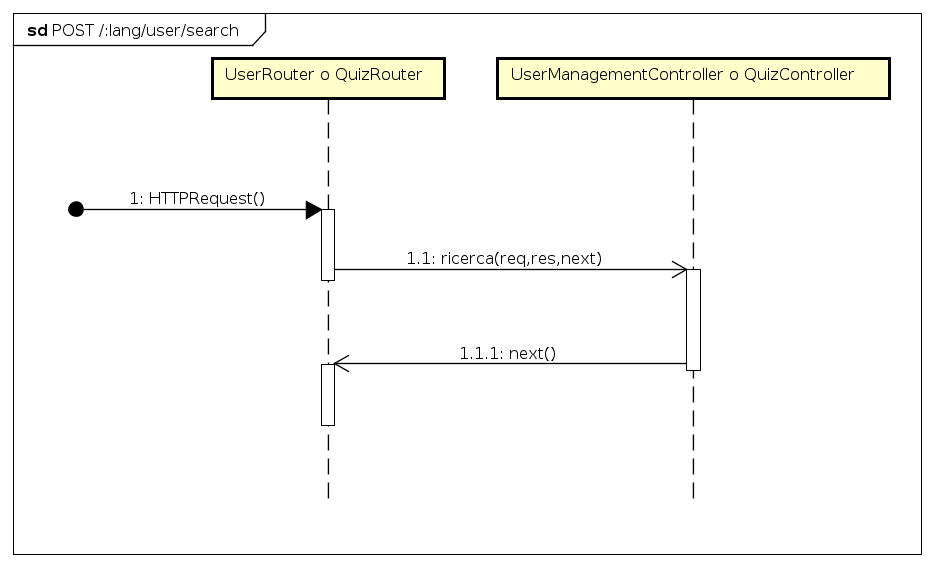
\includegraphics[scale=0.45]{UML/DiagrammiDiSequenza/Back-end/POST__lang_user_search.png}
	\caption{POST /:lang/user/search}
\end{figure}
\FloatBarrier

\item \textbf{Fallimento}
% descrizione diagramma e UML
\end{itemize}

\paragraph{GET /:lang/user/search/:userId}
\begin{itemize}
\item \textbf{Successo}
% descrizione diagramma e UML

\textbf{Descrizione}: lo \texttt{UserRouter} gestisce la richiesta \textit{REST\ped{G}} del Front-End passando il controllo allo \texttt{UserManagementController}; viene poi invocato il metodo\\ \texttt{getInfo(req,res,next)} che ritorna tutte le informazioni riguardanti l'utente.

\begin{figure}[ht]
	\centering
	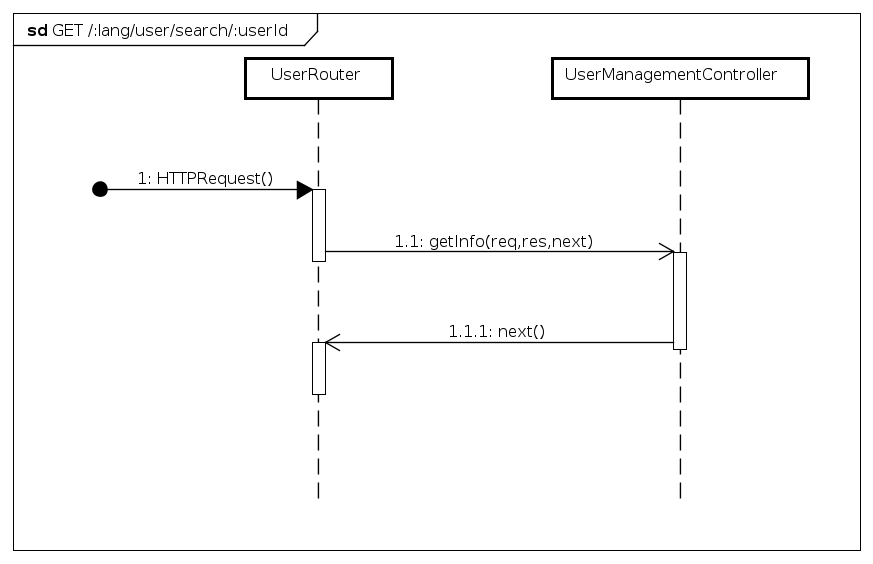
\includegraphics[scale=0.45]{UML/DiagrammiDiSequenza/Back-end/GET__lang_user_search__userId.png}
	\caption{GET /:lang/user/search/:userId}
\end{figure}
\FloatBarrier

\item \textbf{Fallimento}
% descrizione diagramma e UML
\end{itemize}

\paragraph{GET /:lang/user/search/:quizId}
\begin{itemize}
\item \textbf{Successo}
% descrizione diagramma e UML

\textbf{Descrizione}: il \texttt{QuizRouter} gestisce la richiesta \textit{REST\ped{G}} del Front-End passando il controllo al \texttt{QuizController}; viene poi invocato il metodo\\ \texttt{searchQuiz(req,res,next)} che ritorna tutti i questionari ricercati.

\begin{figure}[ht]
	\centering
	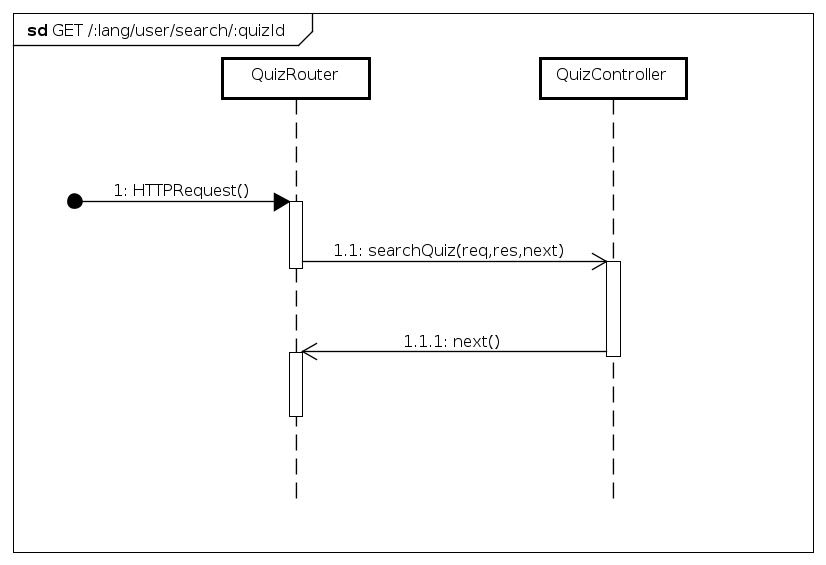
\includegraphics[scale=0.45]{UML/DiagrammiDiSequenza/Back-end/GET__lang_user_search__quizId.png}
	\caption{GET /:lang/user/search/:quizId}
\end{figure}
\FloatBarrier

\item \textbf{Fallimento}
% descrizione diagramma e UML
\end{itemize}
